%%%%%%%%%%%%%%%%%%%%%%%%%%%%%%%%%%%%%%%%%
% Short Sectioned Assignment
% LaTeX Template
% Version 1.0 (5/5/12)
%
% This template has been downloaded from:
% http://www.LaTeXTemplates.com
%
% Original author:
% Frits Wenneker (http://www.howtotex.com)
%
% License:
% CC BY-NC-SA 3.0 (http://creativecommons.org/licenses/by-nc-sa/3.0/)
%
%%%%%%%%%%%%%%%%%%%%%%%%%%%%%%%%%%%%%%%%%

%----------------------------------------------------------------------------------------
%	PACKAGES AND OTHER DOCUMENT CONFIGURATIONS
%----------------------------------------------------------------------------------------

\documentclass[paper=a4, fontsize=11pt]{scrartcl} % A4 paper and 11pt font size

\usepackage[T1]{fontenc} % Use 8-bit encoding that has 256 glyphs
\usepackage{fourier} % Use the Adobe Utopia font for the document - comment this line to return to the LaTeX default
\usepackage[english]{babel} % English language/hyphenation
\usepackage{amsmath,amsfonts,amsthm} % Math packages

\usepackage{graphicx}

\usepackage{sectsty} % Allows customizing section commands
\allsectionsfont{\centering \normalfont\scshape} % Make all sections centered, the default font and small caps

\usepackage[procnames]{listings}

\usepackage{fancyhdr} % Custom headers and footers
\pagestyle{fancyplain} % Makes all pages in the document conform to the custom headers and footers
\fancyhead{} % No page header - if you want one, create it in the same way as the footers below
\fancyfoot[L]{} % Empty left footer
\fancyfoot[C]{} % Empty center footer
\fancyfoot[R]{\thepage} % Page numbering for right footer
\renewcommand{\headrulewidth}{0pt} % Remove header underlines
\renewcommand{\footrulewidth}{0pt} % Remove footer underlines
\setlength{\headheight}{13.6pt} % Customize the height of the header

\numberwithin{equation}{section} % Number equations within sections (i.e. 1.1, 1.2, 2.1, 2.2 instead of 1, 2, 3, 4)
\numberwithin{figure}{section} % Number figures within sections (i.e. 1.1, 1.2, 2.1, 2.2 instead of 1, 2, 3, 4)
\numberwithin{table}{section} % Number tables within sections (i.e. 1.1, 1.2, 2.1, 2.2 instead of 1, 2, 3, 4)

\setlength\parindent{0pt} % Removes all indentation from paragraphs - comment this line for an assignment with lots of text

%----------------------------------------------------------------------------------------
%	TITLE SECTION
%----------------------------------------------------------------------------------------

\newcommand{\horrule}[1]{\rule{\linewidth}{#1}} % Create horizontal rule command with 1 argument of height

\title{	
\normalfont \normalsize 
\textsc{BRSU} \\ [25pt] % Your university, school and/or department name(s)
\horrule{0.5pt} \\[0.4cm] % Thin top horizontal rule
\huge Neural Networks\\Assignment 4 \\ % The assignment title
\horrule{2pt} \\[0.5cm] % Thick bottom horizontal rule
}

\author{Bastian Lang} % Your name

\date{\normalsize\today} % Today's date or a custom date

\begin{document}

\maketitle % Print the title

\newpage

\section{Outline}

\subsection{Statistical Nature of the Learning Process}

\begin{itemize}
	\item Bias/Variance Dilemma
\end{itemize}

\subsection{Statistical Learning Theory}
\begin{itemize}
	\item Some Basic Definitions
	\begin{itemize}
		\item Convergence in probability
		\item Supremum and infimum
		\item Empirical risct functional
		\item Strict Consistency
	\end{itemize}
	\item Principle of Empirical Risk Minimization
	\item VC Dimension
	\item Example 2.1
	\item Example 2.2
	\item Example 2.3
	\item Importance of the VC dimension and its Estimation
	\begin{itemize}
		\item VC dimension of an arbitrary feedforward network using heaviside functions is O(W log W) where W is the total number of free parameters in the network.
		\item The VC dimension of a MLP using sigmoid functions is $O(W^2)$, where W is the number of free parameters.
	\end{itemize}
	\item Constructive Distribution-free Bounds on the Generalization Ability of Learning Machines
	\item Structural Risk Minimization
\end{itemize}

\subsection{Probably Approximately Correct Model of Learning}
\begin{itemize}
	\item Sample Complexity
	\item Computational Complexity
\end{itemize}

\section{Consider the space of instances X corresponding to all points in the x, y plane. Give the VC
dimension of the following hypothesis spaces:}

\subsection{Hr = the set of all rectangles in the x,y plane. i.e. Hr = $\{((a<x<b) \land(c<y<d)) | a, b, c, d \in IR\}$}
4

\subsection{Hc = the set of all circles in the x,y plane. Points inside the circle are classified as positive examples.}
3

\subsection{Ht = the set of all triangle in the x,y plane. Points inside the triangle are classified as positive examples.}
7

\section{Write a consistent learner for $H_r$ from last Exercise (i.e. $H_r = \{((a < x < b)\land(c < y < d)) | a, b, c, d \in IR \}$ ). Generate a variety of target concept rectangles at random, corresponding to different rectangles in the plane. Generate random examples of each of these target concepts, based on a uniform distribution of instances within the rectangle from (0,0) to (100, 100). Plot the generalization error as a function of the number of training examples, m. On the same graph, plot the theoretical relationship between e and m, for d = .95. Does theory fit experiment?}

I was not able to solve this exercise due to too many open questions. It took me about three hours to come to the understanding below:\vspace{5mm}

Questions:
\begin{itemize}
	\item Write a consistent learner...
	\begin{itemize}
		\item How does a learner look like? Is it a function that outputs a hypothesis to a given input? Do we use any kind of ANN and use a learning technique?
	\end{itemize}
	\item Generate a variety of target concept rectangles at random, corresponding to different rectangles in the plane.
	\begin{itemize}
		\item How many? (I will choose some number, not that important)
	\end{itemize}
	\item Generate random examples of each of these target concepts, based on a uniform distribution of instances within the rectangle from (0,0) to (100, 100).
	\begin{itemize}
		\item By examples of a target concept you mean a number of points in the plain within this huge rectangle, classified according to the concept?
	\end{itemize}
	\item Plot the generalization error as a function of the number of training examples, m.
	\begin{itemize}
		\item Use a subset of all examples to train a model?
		\item Use varying numbers of training examples for training until the learner is consistent?
	\end{itemize}
	\item plot the theoretical relationship between e and m, for d = .95.
	\begin{itemize}
		\item E is generalization error?
		\item What is D? Confidence?
	\end{itemize}
	\item Does theory fit experiment?
	\begin{itemize}
		\item Which theory?!
	\end{itemize}
\end{itemize}

I created a Python program that creates some (15) rectangles and for every rectangle 50 points. Those points get classified by the rectangles and both rectangles and points get plotted.

\subsection{Python Code}

\begin{lstlisting}
# -*- coding: utf-8 -*-
"""
Created on Sat Oct 31 13:33:38 2015

@author: bastian
"""

from random import *
import matplotlib.pyplot as plt
import matplotlib.patches as patches
import pylab

class Rect:
    def __init__(self, x_low, y_low, x_high, y_high):
        self.x_low = x_low
        self.x_high = x_high
        self.y_low = y_low
        self.y_high = y_high
        
    def classify_points(self, points):
        result = []
        for point in points:
            if ((point[0] >= self.x_low) and (point[0] <= self.x_high) and (point[1] >= self.y_low) and (point[1] <= self.y_high)):
                result.append(Point(point[0], point[1], 1))
            else:
                result.append(Point(point[0], point[1], 0))
        return result
        
class Point:
    def __init__(self, x, y, value):
        self.x = x
        self.y = y
        self.value = value

def create_random_point(lower_bound, upper_bound):
    return randint(lower_bound, upper_bound)
    
    
def create_random_rectangle():
    x = []
    y = []
    x.append(create_random_point(0, 100))
    x.append(create_random_point(0, 100))
    y.append(create_random_point(0, 100))
    y.append(create_random_point(0, 100))
    
    if x[0] < x[1]:
        x_low = x[0]
        x_high = x[1]
    else:
        x_low = x[1]
        x_high = x[0]
    if y[0] < y[1]:
        y_low = y[0]
        y_high = y[1]
    else:
        y_low = y[1]
        y_high = y[0]
    
    return Rect(x_low, y_low, x_high, y_high)
    
def create_uniformly_distributed_points(number_of_points):
    result = []
    for i in range(number_of_points):
        result.append((create_random_point(0,100), create_random_point(0,100)))     
    return result

def create_rectangles(number_of_rectangles):
    result = []
    for i in range(number_of_rectangles):
        result.append(create_random_rectangle())
    return result
    
def add_rectangle_to_plot(axis, rectangle):
    axis.add_patch(
        patches.Rectangle(
            ((rectangle.x_high - rectangle.x_low) / 2, (rectangle.y_high - rectangle.y_low) / 2),
            rectangle.x_high - rectangle.x_low,
            rectangle.y_high - rectangle.y_low,
            alpha = 0.1
            )
        )

def classify_random_points_with_random_rectangles(rectangles, number_of_points_per_rectangle): 
    classified_points = []
    for rectangle in rectangles:
        points = create_uniformly_distributed_points(number_of_points_per_rectangle)
        classified_points.extend(rectangle.classify_points(points))
    return classified_points


rectangles = create_rectangles(15)
classified_points = classify_random_points_with_random_rectangles(rectangles, 50)
fig1 = plt.figure()

ax1 = fig1.add_subplot(111, aspect='equal')

for rectangle in rectangles:
    add_rectangle_to_plot(ax1, rectangle)
#print classified_points
for point in classified_points:
    #print point
    if point.value == 1:
        ax1.plot(point.x, point.y, 'r+')
    else:
        ax1.plot(point.x, point.y, 'b.')

pylab.ylim([0,100])
pylab.xlim([0,100])

pylab.savefig('ex3.png')
\end{lstlisting}

\begin{figure}[ht]
	\centering
  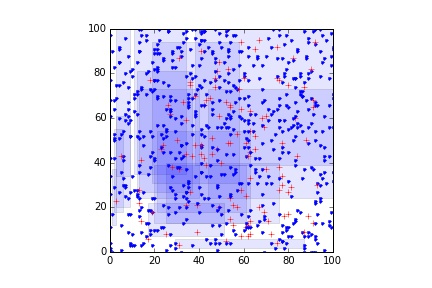
\includegraphics[width=0.7\textheight]{ex3.jpg}
	\caption{Output}
	\label{fig1}
\end{figure}

\section{Rephrase the Ex2.21 of chapter 2 from Haykin's book in such way that the next students will understand it better.}


\end{document}